\wip
\section{Spannungsabfall}
Herkömmliche CAT5-Ethernetkabel wurden ursprünglich nicht für die Übertragung großer elektrischer Leistungen entwickelt und besitzen daher Leitungen mit einem sehr geringen Ader-Durchmesser.
Aufgrund dieser Gegebenheit kann es bei weiten Entfernungen oder großen übertragenen Leistungen zu abnormal hohen Spannungsabfällen kommen.
Um die Anlage in dieser Hinsicht zu überprüfen werden sämtliche Spannungsabfälle und die damit verbundenen Verlustleistungen bei maximaler Belastung durch die Stationen berechnet.
Zur Berechnung der Spannungsabfälle sind folgende Angaben verwendet worden.
\begin{itemize}
	\item Es werden vier Stationen über \ac{poe} versorgt.
	Die Stationen sind nach Abbildung \crossref{fig:poe-verdrahtung} miteinander verdrahtet.
	\item Jede Station hat einen maximalen Leistungsverbrauch von 12 W.
	\item Das Ethernetkabel zwischen den Stationen hat jeweils eine Länge von 10 m.
	\item Der Querschnitt einer Ader des Ethernet-Kabels beträgt 0.128 mm\textsuperscript{2} \cite[vgl.][]{lapp-cat5-datasheet}.
	\item Am PSE wird eine Spannung von 30 V in das Netz eingespeist.
\end{itemize}
\begin{figure}[H]
	\centering
	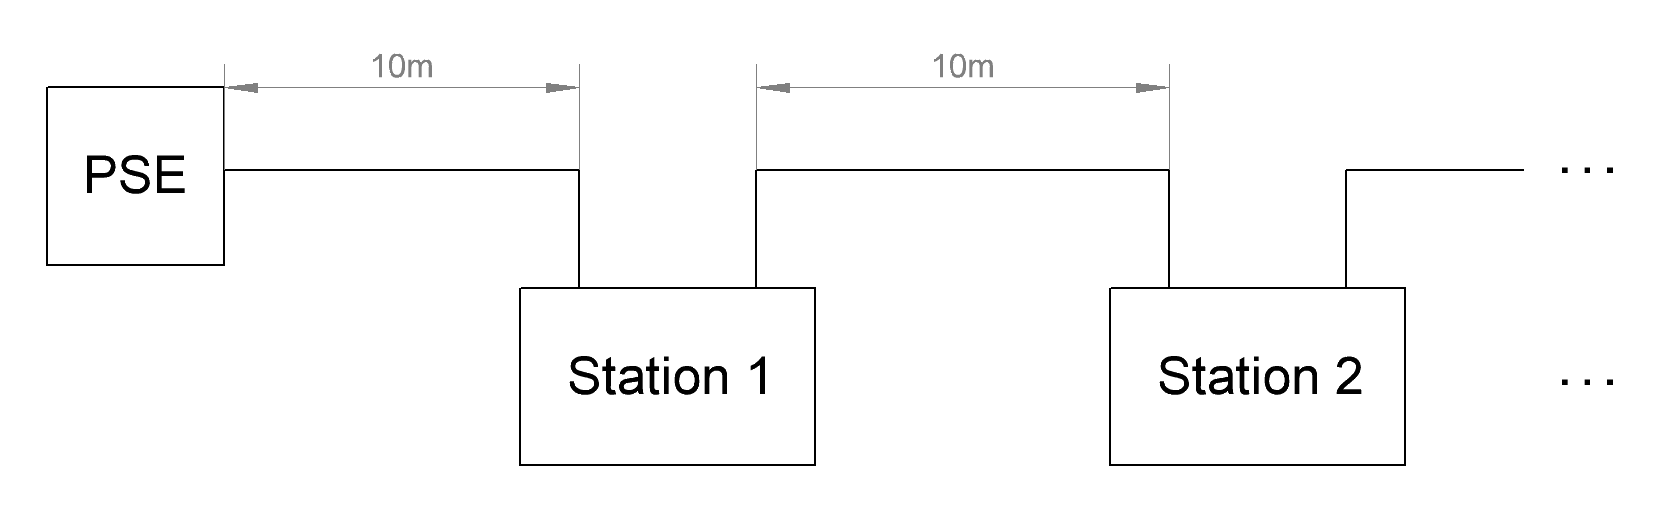
\includegraphics[width=.9\linewidth]{images/berechnung/poe_verdrahtung.png}
	\caption{Verdrahtungsschema}
	\label{fig:poe-verdrahtung}
\end{figure}
Der Leitungswiderstand eines Adernpaares des Ethernetkabels beträgt nach der allgemeinen Drahtwiderstandsformel $R_{Ltg}=\frac{l}{\gamma\cdot A}=0.686\Omega$.
Je nach verwendeter PoE-Type werden mehrere Adernpaare parallel geschaltet, um den Leitungswiderstand zu veringern.
Anhand der oben beschriebenen Verdrahtung ergeben sich folgende Ersatzschaltungen:
\begin{figure}[H]
	\centering
	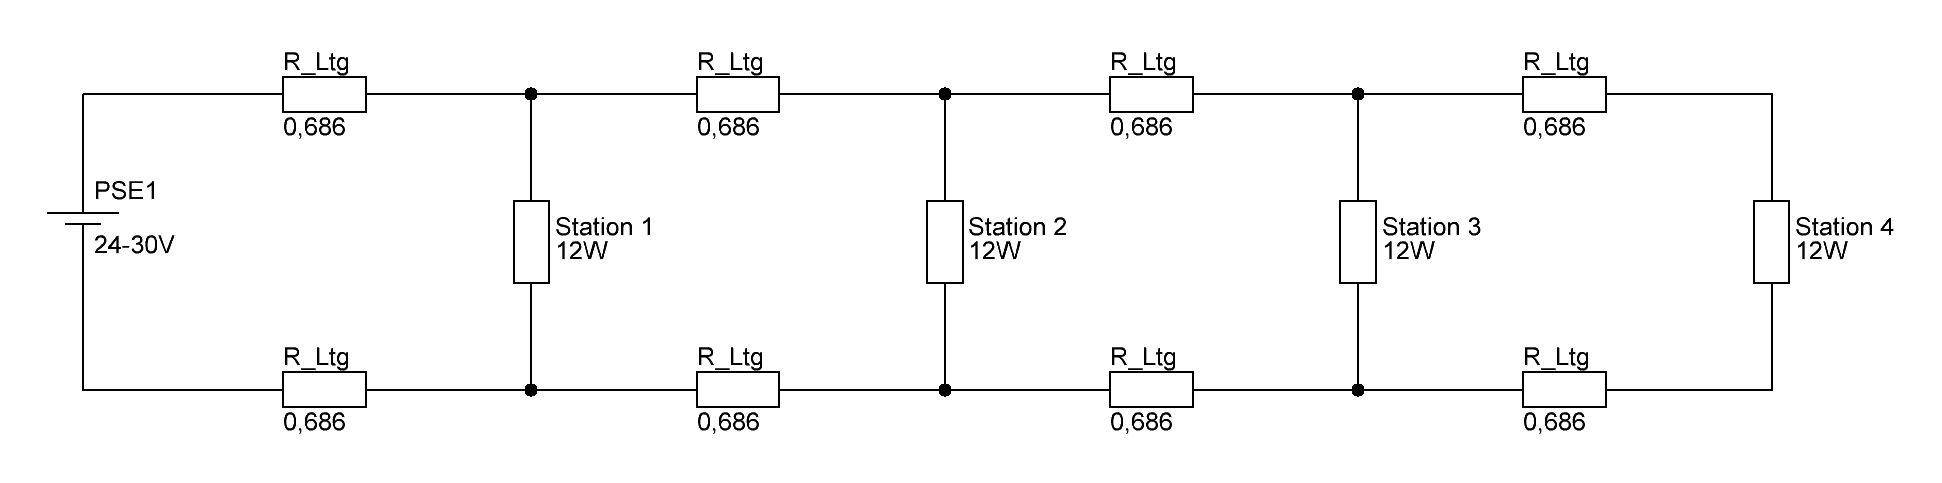
\includegraphics[width=\linewidth]{images/berechnung/poe2pair.png}
	\caption{Ersatzschaltung PoE Type 1 und 2}
\end{figure}
\begin{figure}[H]
	\centering
	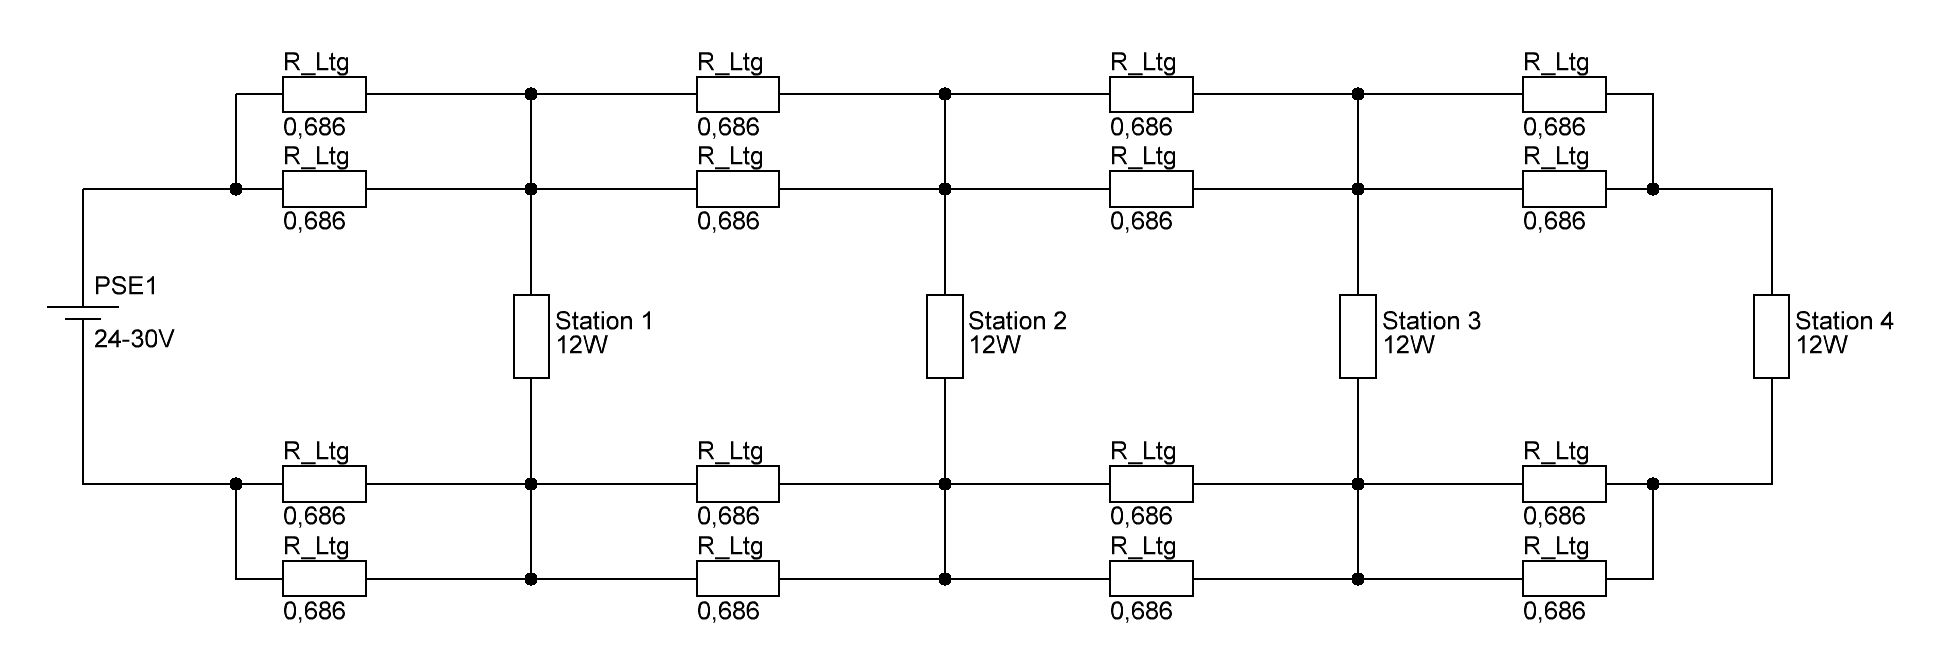
\includegraphics[width=\linewidth]{images/berechnung/poe4pair_neu.jpg}
	\caption{Ersatzschaltung PoE Type 3 und 4}
\end{figure}
U\textsubscript{n}\dots Spannung an Station n, I\textsubscript{n}\dots Strom durch Station n, U\textsubscript{0}\dots Quellenspannung;\par
Anhand dieser Ersatzschaltung ergeben sich folgende Berechnungsformeln:
\begin{align}
	U_1 &= U_0-2\cdot R_{Ltg}\cdot (I_1+I_2+I_3+I_4)\\
	U_2 &= U_1-2\cdot R_{Ltg}\cdot (I_2+I_3+I_4)\\
	U_3 &= U_2-2\cdot R_{Ltg}\cdot (I_3+I_4)\\
	U_4 &= U_3-2\cdot R_{Ltg}\cdot I_4\\
	12W &= U_1\cdot I_1\\
	12W &= U_2\cdot I_2\\
	12W &= U_3\cdot I_3\\
	12W &= U_4\cdot I_4
\end{align}
Zur Lösung dieses Gleichungssystems wurde das CAS-System Maxima verwendet.
Die Eingabe sieht wie folgt aus:
\begin{figure}[H]
	\centering
	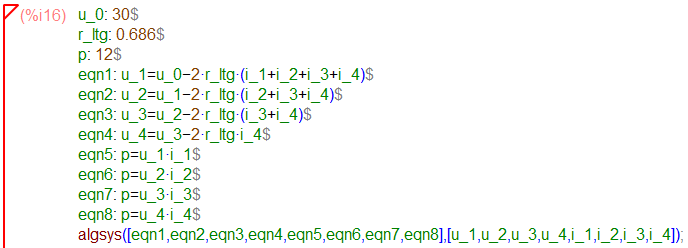
\includegraphics[width=.9\linewidth]{images/berechnung/max_2pair_30V.png}
	\caption{Eingabe wxMaxima Type 1 \& 2}
\end{figure}
Die Lösungen für das Gleichungssystem werden vom Programm in Textform zurückgegeben.
Das Programm findet neben der relevanten Lösung noch einige komplexe Lösungen für das Gleichungssystem.
Diese werden hier wegen Platzgründen und niedriger Relevanz weggelassen.
\begin{table}[H]
	\centering
	\begin{tabular}{|r|c|c|c|c|}
		\hline
		&\multicolumn{2}{c|}{Type 1 \& 2}&\multicolumn{2}{c|}{Type 3 \& 4}\\\cline{2-5}
		&U&I&U&I\\
		\midrule
		Station 1&27.35 V&438 mA&28.81 V&416 mA\\\hline
		Station 2&25.30 V&474 mA&27.91 V&430 mA\\\hline
		Station 3&23.90 V&502 mA&27.31 V&439 mA\\\hline
		Station 4&23.19 V&517 mA&27.00 V&444 mA\\
		\hline
	\end{tabular}
	\caption{Maxima-Ergebnisse Spannungsabfall}
\end{table}
Man sieht: Der Spannungsabfall ist wie erwartet bei Type 3 und 4 etwa halb so groß wie bei Type 1 und 2.
